\documentclass[UTF8,a4paper,zihao=-4,fontset=none,oneside]{ctexart}

\newif\ifprofessional
\newif\ifreview

% ======================== 待编辑信息 ========================
\professionalfalse % 默认\professionalfalse为学术硕士；改为\professionaltrue切换为专业硕士
\reviewfalse %默认\reviewfalse为开题报告；改为\professionaltrue切换为文献综述

% 题目，不超过25个汉字
\newcommand{\ReportTitle}{控制系统………………\\……………分析}

\newcommand{\Classification}{×××××}		%中图分类号
\newcommand{\StudentNumber}{SY2503×××}	%学号
\newcommand{\AuthorName}{高××}			%学生姓名
\newcommand{\MajorName}{控制科学与工程}	%专业名称
\newcommand{\SupervisorName}{张××}		%导师姓名
\newcommand{\SupervisorTitle}{教授}		%导师职称
\newcommand{\SecondSupervisor}{李××} 	%第二导师姓名，可留空
\newcommand{\SecondSupervisorTitle}{副教授}%第二导师职称


% ======================================================================
\usepackage[left=31.8mm,right=25.9mm,top=25.4mm,bottom=25.4mm,headheight=19bp,headsep=3.7mm,footskip=8mm]{geometry}
\usepackage{iftex}
\usepackage{fontspec}
\usepackage{xeCJK}
\usepackage{etoolbox}
\usepackage{setspace}
\usepackage{fancyhdr}
\usepackage{booktabs}
\usepackage{array}
\usepackage{tabularx}
\usepackage{tikz}
\usetikzlibrary{arrows.meta,positioning}
\usepackage{amsmath}
\usepackage{newtxmath}
\usepackage{chngcntr}
\usepackage{caption}
\usepackage{graphicx}
\usepackage[numbers,square,super,sort&compress]{natbib}
\usepackage[hidelinks]{hyperref}


% 字体选择
\IfFontExistsTF{Times New Roman}{\setmainfont{Times New Roman}}{\setmainfont{TeX Gyre Termes}\PackageWarning{main}{Times New Roman unavailable; using TeX Gyre Termes}}
\IfFontExistsTF{SimSun}{%
  \setCJKmainfont[AutoFakeBold=2]{SimSun}%
  \setCJKfamilyfont{zhsong}[AutoFakeBold=2]{SimSun}%
}{%
  \setCJKmainfont[BoldFont=FandolSong-Bold]{FandolSong-Regular}%
  \setCJKfamilyfont{zhsong}[BoldFont=FandolSong-Bold]{FandolSong-Regular}%
  \PackageWarning{main}{SimSun unavailable; using FandolSong-Regular with FandolSong-Bold}%
}
\IfFontExistsTF{SimHei}{%
  \setCJKsansfont{SimHei}%
  \setCJKfamilyfont{zhhei}{SimHei}%
}{%
  \setCJKsansfont[BoldFont=FandolHei-Bold]{FandolHei-Regular}%
  \setCJKfamilyfont{zhhei}[BoldFont=FandolHei-Bold]{FandolHei-Regular}%
  \PackageWarning{main}{SimHei unavailable; using FandolHei-Regular with FandolHei-Bold}%
}
\IfFontExistsTF{STXingkai}{\setCJKfamilyfont{kai}{STXingkai}}{%
  \IfFontExistsTF{KaiTi}{\setCJKfamilyfont{kai}{KaiTi}\PackageWarning{main}{STXingkai unavailable; using KaiTi}}{%
    \setCJKfamilyfont{kai}{FandolKai-Regular}%
    \PackageWarning{main}{STXingkai and KaiTi unavailable; using FandolKai-Regular}%
  }%
}
\providecommand{\songti}{\CJKfamily{zhsong}}
\providecommand{\heiti}{\CJKfamily{zhhei}}
\newcommand{\xingkai}{\CJKfamily{kai}}
\setCJKfamilyfont{coverhei}[AutoFakeBold=3]{SimHei}
\setCJKfamilyfont{fangsonggb}[Path=fonts/]{FangSong_GB2312.ttf}
\newcommand{\fangsonggb}{\CJKfamily{fangsonggb}}
\newfontfamily\tnr{Times New Roman}

\setlength{\parindent}{2em}
\setlength{\parskip}{0pt}
\setstretch{1}
\pagestyle{fancy}
\fancyhf{}
\fancyhead[C]{\songti\fontsize{12bp}{18bp}\selectfont 北京航空航天大学自动化科学与电气工程学院}
\fancyfoot[C]{\thepage}
\renewcommand{\footrulewidth}{0pt}
\fancypagestyle{plain}{\fancyhf{}\fancyhead[C]{\songti\fontsize{12bp}{18bp}\selectfont 北京航空航天大学自动化科学与电气工程学院}\fancyfoot[C]{\thepage}\renewcommand{\headrulewidth}{0.4pt}}

% ctex 自带标题机制，避免与 titlesec 同时改写标题格式。
\ctexset{
  section={format=\heiti\fontsize{15bp}{22bp}\selectfont,name={},number=\thesection.,beforeskip=1.1em,afterskip=0.5em,indent=0pt},
  subsection={format=\songti\bfseries\fontsize{14bp}{21bp}\selectfont,name={},number=\thesubsection,beforeskip=0em,afterskip=0.5em,indent=1em},
  subsubsection={format=\songti\bfseries\fontsize{12bp}{18bp}\selectfont,name={},number=\thesubsubsection,beforeskip=0.6em,afterskip=0.25em,indent=0pt}
}
\setcounter{secnumdepth}{3}
\renewcommand{\thesection}{\arabic{section}}
\renewcommand{\thesubsection}{\thesection.\arabic{subsection}}
\renewcommand{\thesubsubsection}{\thesubsection.\arabic{subsubsection}}
\counterwithin{equation}{section}
\counterwithin{figure}{section}
\counterwithin{table}{section}
\captionsetup{font=small,labelfont=bf,justification=centering}
\renewcommand{\bibsection}{\section{主要参考文献}}
\setlength{\bibsep}{0pt}
\renewcommand{\bibfont}{\songti\fontsize{12bp}{14.4bp}\selectfont\raggedright}
\newcommand{\第二导师行}{\ifdefempty{\SecondSupervisor}{}{ &\SecondSupervisor\quad\SecondSupervisorTitle\\}}
\bibliographystyle{def/GBT7714-2015-NoWarning}

\begin{document}
\pagenumbering{gobble}
\thispagestyle{empty}

\begin{center}
\begin{minipage}{0.92\textwidth}
\CJKfamily{coverhei}\bfseries\fontsize{12bp}{18bp}\selectfont
\begin{tabular}{@{}l@{}l@{}}
	\makebox[5em][s]{中图分类号}：&\Classification\\
	\makebox[5em][s]{学号}：&\StudentNumber\\
\end{tabular}
\end{minipage}
\vspace{25mm}


\includegraphics[width=0.55\textwidth]{pic/logo-buaa}\par
{\xingkai\fontsize{42pt}{50pt}\selectfont\ifreview\ifprofessional 专业硕士学位文献综述 \else \ziju{0.3}硕士文献综述\fi\else\ifprofessional 专业硕士学位开题报告\else 硕士开题报告\fi\fi\par}
\vspace{20mm}

\begin{minipage}[c][50mm][c]{\textwidth}
\centering
{\setstretch{1}\songti\bfseries\fontsize{32bp}{42bp}\selectfont
\parbox{\linewidth}{\centering\ReportTitle\par}}
\end{minipage}

\begin{minipage}{100mm}
\setstretch{1}
\heiti\fontsize{14bp}{22bp}\selectfont
\renewcommand{\arraystretch}{1.45}
\vspace{3\baselineskip}
\begin{tabular}{@{}>{\hspace{1em}\ziju{0.15}}p{7em}p{\dimexpr\linewidth-4.5em-2\tabcolsep\relax}@{}}
	作者姓名&\AuthorName\\
	学科专业&\MajorName\\
	指导教师&\SupervisorName\quad\SupervisorTitle\\
	\第二导师行
	培养院系&自动化科学与电气工程学院\\
\end{tabular}
\end{minipage}
\end{center}
\clearpage
\pagenumbering{arabic}
\setcounter{page}{1}

\ifreview
\section{} %这边应该不要编号(?)
% 中文摘要
\noindent
{\heiti\fontsize{12bp}{18bp}\selectfont 摘要：}
{\fangsonggb\fontsize{12bp}{18bp}\selectfont
	这里填写中文摘要内容。摘要控制在400字左右。
	\par}

\vspace{0.5\baselineskip}

\noindent
{\heiti\fontsize{12bp}{18bp}\selectfont 关键词：}%
{\fangsonggb\fontsize{12bp}{18bp}\selectfont
	关键词一；关键词二；关键词三；关键词四；关键词五
	\par}

\vspace{1.5\baselineskip}

% 英文摘要
\noindent
{\tnr\bfseries\fontsize{12bp}{18bp}\selectfont Abstracts: }%
{\tnr\fontsize{12bp}{18bp}\selectfont
	This is the English abstract. The main text of the abstract is set in
	12 bp Times New Roman.
	\par}

\vspace{0.5\baselineskip}

\noindent
{\tnr\bfseries\fontsize{12bp}{18bp}\selectfont Key words: }%
{\tnr\fontsize{12bp}{18bp}\selectfont
	keyword one; keyword two; keyword three; keyword four; keyword five
	\par}
\newpage
\section{文献概述}
包括：对所述研究方向阅读文献的概述\cite{guo2025deepseek}。
\section{基本研究现状与发展趋势}

所述研究方向的基本研究现状与发展趋势，含主要研究的若干分支，每个分支的理论/方法/方案//技术研究的现状，关键问题已解决的程度与尚待解决的难点，未来发展的趋势等，按参考文献书写格式标注参考文献\cite{JSJY20260928003}
\section{结论}
这一部分是结论，参考图是\ref{fig:example}。

\begin{figure}[htbp]
	\centering
	
\includegraphics[width=0.8\textwidth]{pic/zongshu/example.png}
	\caption{这是例图。}\label{fig:example}
\end{figure}
\bibliography{ref/zongshu/reference}
\else
\section{论文选题依据}
这一部分是论文选题依据。And this is English example.
\subsection{研究背景与意义}
说明问题背景、研究价值和选题依据\cite{guo2025deepseek}。

\subsection{国内外研究现状}
概述相关方向的代表性工作、方法和不足。

\section{论文研究方案}
这一部分是论文研究方案。
\subsection{研究目标及研究内容}
用可检验的目标概括研究范围，再分点说明拟完成的研究内容。

\subsection{拟解决的关键问题及难点}
说明关键科学或工程问题、主要难点及其与研究目标的关系。

\subsection{拟采用的研究方法、技术路线、实验方案及预期的新意/创新}
依次交代研究方法、技术路线、实验或验证方案，以及有依据的预期创新点。

图\ref{fig:route}为可替换的自绘技术路线示意。公式\eqref{eq:placeholder}中的$N$为样本数，$x_i$和$y_i$为第$i$个样本及其目标值，$\theta$为模型参数，$\ell$为单样本损失\cite{JSJY20260928003}。
\begin{figure}[htbp]
\centering
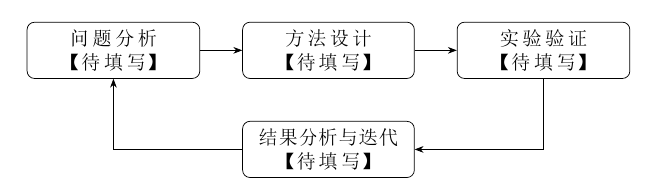
\includegraphics[width=0.8\textwidth]{pic/kaiti/flowchart.png}
\caption{技术路线示例框图（请替换节点内容）}\label{fig:route}
\end{figure}

\begin{equation}
J(\theta)=\frac{1}{N}\sum_{i=1}^{N}\ell\bigl(f_{\theta}(x_i),y_i\bigr)
\label{eq:placeholder}
\end{equation}
\section{预期达到的目标及考核指标}
这一部分是预期达到的目标及考核指标。
\begin{table}[htbp]
	\centering
	\caption{预期目标与考核指标}
	\label{tab:targets}
	
	\begin{tabularx}{0.96\textwidth}{
			>{\centering\arraybackslash}p{0.2\textwidth}
			>{\centering\arraybackslash}X
			>{\centering\arraybackslash}p{0.25\textwidth}
		}
		\toprule
		目标项 & 指标及测量方式 & 预期值\\
		\midrule
		【目标一】 & 【填写可测量的指标与验证方法】 & 【待填写】\\
		【目标二】 & 【填写可测量的指标与验证方法】 & 【待填写】\\
		\bottomrule
	\end{tabularx}
\end{table}

表\ref{tab:targets}中的内容仅供排版参考。
\section{论文工作计划}
这一部分是论文工作计划。
\begin{table}[htbp]
	\centering
	\caption{论文工作计划}
	\label{tab:plan}
	
	\begin{tabularx}{0.96\textwidth}{
			>{\centering\arraybackslash}p{0.25\textwidth}
			>{\centering\arraybackslash}X
		}
		\toprule
		起止年月 & 工作内容与阶段成果\\
		\midrule
		20XX年XX月—20XX年XX月 & 【文献调研、问题细化等】\\
		20XX年XX月—20XX年XX月 & 【方法设计与阶段验证等】\\
		20XX年XX月—20XX年XX月 & 【实验、总结与论文撰写等】\\
		\bottomrule
	\end{tabularx}
\end{table}
\bibliography{ref/kaiti/reference}
\fi

\end{document}

